\chapter{Dynamic Optimisation}
\label{cha:do}

This chapter deals with dynamic optimisation in general. The chapter
starts with several dynamic optimisation problem definitions. Finally,
this chapter ends with the NLP problem formulation. 

\section{Optimisation Problem Statement}
\label{sec:ops}

The objective of dynamic optimisation is to determine, in open loop
control, a set of time dependent decision variables (pressure,
temperature, flow rate, current, heat duty,~\ldots) that optimise a
given performance index (or cost functional or optimisation
criterion)(cost, time, energy, selectivity,~\ldots) subject to
specified constraints (safety, environmental and operating
constraints). Optimal control refers to the determination of the best
time-varying profiles in closed loop control.

\subsection{Cost Functional}
\label{sec:cf}

The performance index (cost functional or optimisation criterion) can
in general be written in one of three forms as follows:
\paragraph{Bolza form}
\begin{equation}
\mf{J}(\ve{u}(t),\ve{p},t_{f}) = \mf{G}(\ve{x}(t_{f}),\ve{p},t_{f}) +
\int_{t_{0}}^{t_{f}}\mf{F}(\ve{x}(t),\ve{u}(t),\ve{p},t)\dt
\label{eq:bolza} 
\end{equation} 
\paragraph{Lagrange form}
\begin{equation}
\mf{J}(\ve{u}(t),\ve{p},t_{f}) =
\int_{t_{0}}^{t_{f}}\mf{F}(\ve{x}(t),\ve{u}(t),\ve{p},t)\dt
\label{eq:lagrange}
\end{equation} 
\paragraph{Mayer form}
\begin{equation}
\mf{J}(\ve{u}(t),\ve{p},t_{f}) = \mf{G}(\ve{x}(t_{f}),\ve{p},t_{f})
\label{eq:mayer} 
\end{equation}where
\begin{description}
\item[$\mf{J}(\cdot)$] -- optimisation criterion,
\item[$\mf{G}(\cdot)$] -- component of objective function evaluated at
  final conditions, 
\item[$\int_{t_{0}}^{t_{f}}\mf{F}(\cdot)\dt$] -- component of the
  objective 
  function evaluated over a period of time, 
\item[$\ve{x}(t)$] --  vector of state variables,
\item[$\ve{u}(t)$] -- vector of control variables,
\item[$\ve{p}$] -- vector of time independent parameters,
\item[$t_0,t_{f}$] -- initial and final times.
\end{description}
Note that all three forms are interchangeable and can be derived one
from another. In the sequel, Mayer form will be used.
 
\subsection{Process Model Equations}
\label{sec:pme}

The behaviour of many of processes can in general be described either
by a set of ordinary differential equations (ODE's) or by a set of
differential-algebraic equations (DAE's) as follows:
\begin{equation}
\ve{M\dot{x}}(t) = \ve{f}(\ve{x}(t),\ve{u}(t),\ve{p},t), \quad
\ve{x}(t_{0}) = \ve{x}_{0} \quad \textnormal{over} \quad t_{0} \leq t
\leq t_{f} \label{eq:process} 
\end{equation} with initial condition for states $\ve{x}_{0}$ which may
also be a function of some time independent parameters. Here $\ve{M}$
is a constant mass matrix. This ODE or DAE system forms equality constraint
in optimal control problem. 

\subsection{Constraints}
\label{sec:cons}

Constraints to be accounted for typically include
equality and inequality infinite dimensional, interior-point, and
terminal-point constraints~\cite{goh88}. Moreover, they may be written
in the following canonical form similar to the cost
form~\eqref{eq:mayer}: 
\begin{equation}
\mf{J}_{i}(\ve{u}(t),\ve{p},t_i) = \mf{G}_{i}(\ve{x}(t_{i}),\ve{p},t_i) 
\label{eq:constraints} 
\end{equation} where $t_i \leq t_f$, $i=1,\ldots,nc$, and $nc$ is
the number of constraints.

\section{Optimal Control Problem Solutions}
\label{sec:ocps}

There are several approaches that can solve optimal control problems.
These can be divided into analytical methods that have been used
originally and numerical methods preferred nowadays. In this work only
numerical methods are considered.

The numerical methods used for the solution of dynamic optimisation
problems can then be grouped into two categories: indirect and direct
methods. In this work only direct methods are considered. In this
category, there are two strategies: sequential method and simultaneous
method. The sequential strategy, often called control vector
parameterisation (CVP), consists in an approximation of the control
trajectory by a function of only few parameters and leaving the state
equations in the form of the original ODE/DAE system~\cite{goh88}. In
the simultaneous strategy often called total discretisation method,
both the control and state variables are discretised using polynomials
(e.g., Lagrange polynomials) of which the coefficients become the
decision variables in a much larger NLP problem~\cite{cut87}.
Implementation of this method is subject of this work.

Next section reviews the general NLP formulation for optimal control
problems using orthogonal collocation on finite elements method.

\section{NLP Formulation Problem}
\label{sec:nlp-fp}

As mentioned before, the optimal control problem will be solved by
complete parametrisation of both the control and the state profile
vector~\citep{log89,log92}. That means, that the control and state
profiles are approximated by a linear combination of some basis
functions. It is expected here, that the basis functions are known so
only the coefficients of linear combination of these fundamentals have
to be optimised. In addition, each control sequence segment is defined
on time interval, which length itself can be the optimised
variable. Finally, a set of time independent parameters may influence
the process model and can also be optimised. As mentioned
in section {sec:pme}, it is supposed that the optimised dynamic model can
be described either by an ODE system or by an DAE system.

Consider the following general control problem for $t \in
[t_{0},t_{f}]$:
\begin{equation}
\min_{\ve{u}(t),\ve{p}}\{\mf{G}(\ve{x}(t_{f}),\ve{p},t_{f})\}
\label{eq:gencontprob} 
\end{equation}
such that
\begin{gather}
\ve{M\dot{x}}(t) = \ve{f}(\ve{x}(t),\ve{u}(t),\ve{p},t), \quad
\ve{x}(t_{0}) = \ve{x}_{0}(\ve{p})\nonumber\\  
\ve{h}(\ve{x}(t),\ve{u}(t),\ve{p},t) = \ve{0}\nonumber\\ 
\ve{g}(\ve{x}(t),\ve{u}(t),\ve{p},t) \leq \ve{0}\nonumber\\
\ve{x}(t)^{L} \leq \ve{x}(t) \leq \ve{x}(t)^{U}\nonumber\\ 
\ve{u}(t)^{L} \leq \ve{u}(t) \leq \ve{u}(t)^{U}\nonumber\\
\ve{p}^{L} \leq \ve{p} \leq \ve{p}^{U}\nonumber  
\end{gather}with following nomenclature:
\begin{description}
\item [$\ve{h}(\cdot)$] -- equality design constraint vector,
\item [$\ve{g}(\cdot)$] -- inequality design constraint vector,
\item [$\ve{x}(t)^{L},\ve{x}(t)^{U}$] -- state profile bounds, 
\item [$\ve{u}(t)^{L},\ve{u}(t)^{U}$] -- control profile bounds,
\item [$\ve{p}^{L},\ve{p}^{U}$] -- parameter bounds.
\end{description}

In order to derive the NLP problem the differential equations are
converted into algebraic equations using collocation on finite
elements. Residual equations are then formed and solved as a set of
algebraic equations. These residuals are evaluated at the shifted
roots of Legendre polynomials. The procedure is then following:
Consider the initial-value problem over a finite element $i$ with time 
$t\in[\zeta_{i},\zeta_{i+1}]$:
\begin{equation}
\ve{M\dot{x}} = \ve{f}(\ve{x}(t),\ve{u}(t),\ve{p},t) \quad
t\in[t_{0},t_{f}]  
\end{equation}
The solution is approximated by Lagrange polynomials
over element $i,~\zeta_{i}\leq t\leq \zeta_{i+1}$ as follows: 
\begin{gather}
\ve{x}_{K_{x}}(t) = \sum_{j=0}^{K_{x}}\ve{x}_{ij}\phi_{j}(t); \quad
\phi_{j}(t) = \prod_{k=0,j}^{K_{x}}\frac{(t-t_{ik})}{(t_{ij}-t_{ik})}\\
\textrm{in element}~i\qquad i=1,\ldots,\textrm{NE}\nonumber\\  
\ve{u}_{K_{u}}(t) = \sum_{j=1}^{K_{u}}\ve{u}_{ij}\theta_{j}(t); \quad
{\theta_{j}}(t) = \prod_{k=1,j}^{K_{u}}\frac{(t-t_{ik})}{(t_{ij}-t_{ik})}\\
\textrm{in element}~i\qquad i=1,\ldots,\textrm{NE}\nonumber 
\end{gather}
Here $k=0,j$ means $k$ starting form 0 and $k\ne
j$,~\textrm{NE} is the number of elements. Also $\ve{x}_{K_{x}}(t)$ is
a $(K_{x}+1)$th degree piecewise polynomial and $\ve{u}_{K_{u}}(t)$ is
piecewise polynomial of order $K_{u}$. The polynomial approximating
the state $\ve{x}$ takes into account the initial conditions of
$\ve{x}(t)$ for each element $i$. Also, the Lagrange polynomial has the
desirable property that (for $\ve{x}_{K_{x}}(t)$, for example): 
\begin{equation}
\ve{x}_{K_{x}}(t_{ij}) = \ve{x}_{ij}
\end{equation}
which is due to the Lagrange condition
$\phi_{k}(t_{j}) = \delta_{kj}$, where $\delta_{kj}$ is the Kronecker
delta. This polynomial form allows the direct bounding of the states
and controls, e.g., path constraints can be imposed on the problem
formulation.  

\begin{figure}
\begin{minipage}[t]{0.95\linewidth}
\centering
\psfrag{t0}{$\zeta_{i-1}$}
\psfrag{t1}{$\zeta_{i}$}
\psfrag{t2}{$\zeta_{i+1}$}
\psfrag{t3}{$\zeta_{i+2}$}
\psfrag{t}{$\Delta\zeta_{i}$}
\psfrag{x01}{$x_{i-1,0}$}
\psfrag{x02}{$x_{i-1,1}$}
\psfrag{x03}{$x_{i-1,2}$}
\psfrag{x11}{$x_{i,0}$}
\psfrag{x12}{$x_{i,1}$}
\psfrag{x13}{$x_{i,2}$}
\psfrag{x21}{$x_{i+1,0}$}
\psfrag{x22}{$x_{i+1,1}$}
\psfrag{x23}{$x_{i+1,2}$}
\psfrag{xf}{$x_{i+2,0}$}
\psfrag{u02}{$u_{i-1,1}$}
\psfrag{u03}{$u_{i-1,2}$}
\psfrag{u12}{$u_{i,1}$}
\psfrag{u13}{$u_{i,2}$}
\psfrag{u22}{$u_{i+1,1}$}
\psfrag{u23}{$u_{i+1,2}$}
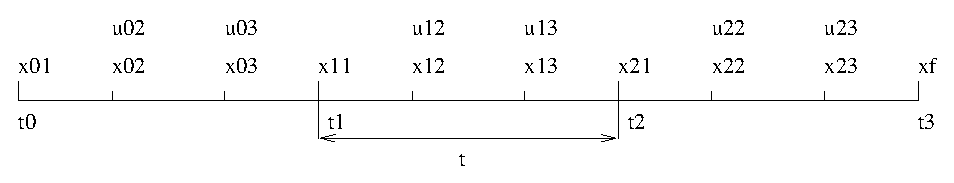
\includegraphics[width=1\textwidth]{pictures/collocation.eps}
\caption[Collocation method on finite elements]{Collocation method on
  finite elements for state profiles, control profiles and element
  lengths ($K_{x} = K_{u} = 2$)} 
\label{fig:colloc}
\end{minipage}
\end{figure}

Using $K = K_{x} = K_{u}$ point orthogonal collocation on finite elements as shown
in Fig.~\ref{fig:colloc}, and by defining the basis functions, so that they
are normalised over the each element $\Delta\zeta_{i}(\tau\in[0,1])$,
one can write the residual equation as follows:
\begin{gather}
\Delta\zeta_{i}\ve{r}(t_{ik}) =
\ve{M}\sum_{j=0}^{K_{x}}\ve{x}_{ij}\dot{\phi_{j}}(\tau_{k}) -
\Delta\zeta_{i}\ve{f}(t_{ik},\ve{x}_{ik},\ve{u}_{ik},\ve{p})\\
i=1,\ldots,\textrm{NE}, \quad j=0,\ldots,K_{x}, \quad k=1,\ldots,K_{x}
\nonumber  
\end{gather}
where $\dot{\phi_{j}}(\tau_{k}) = \dt\phi_{j}/\dt\tau$, and
together with $\phi_{j}(\tau),~\theta_{j}(\tau)$ terms (basis
functions), they are calculated beforehand, since they depend only on
the Legendre root locations. Note that
$t_{ik} = \zeta_{i} + \Delta\zeta_{i}\tau_{k}$. This form is
convenient to work with when the element lengths are included as
decision variables. The element lengths are also used to find possible
points   of discontinuity for the control profiles and to insure that
the integration accuracy is within a numerical tolerance. Additionally,
the continuity of the states is enforced at element endpoints
(interior knots $\zeta_{i},i=2,...,\mathrm{NE}$), but it is allowed that
the control profiles to have discontinuities at these endpoints. Here
\begin{gather}
\ve{x}_{K_{x}}^{i}(\zeta_{i}) = \ve{x}_{K_{x}}^{i-1}(\zeta_{i})\\
i=2,\ldots,\textrm{NE}\nonumber
\end{gather}or
\begin{gather}
\ve{x}_{i0} = \sum_{j=0}^{K_{x}}\ve{x}_{i-1,j}\phi_{j}(\tau=1)\\
i=2,\ldots,\textrm{NE}, \quad j=0,\ldots,K_{x}\nonumber 
\end{gather}
These equations extrapolate the polynomial
$\ve{x}_{K_{x}}^{i-1}(t)$ to the endpoints of its element and provide an
accurate initial conditions for the next element and polynomial
$\ve{x}_{K_{x}}^{i}(t)$. 

At this point a few additional comments concerning construction of the
control profile polynomials must be made. Note that these
polynomials use only $K_{u}$ coefficients per element and are of lower
order than the state polynomials. As a result these profiles are
constrained or bounded only at collocation points. The constraints of
the control profile are carried out by bounding the values of each
control polynomial at both ends of the element. This can be done by
writing the equations: 
\begin{gather}
\ve{u}_{i}^{L} \leq \ve{u}_{K_{u}}^{i}(\zeta_{i}) \leq
\ve{u}_{i}^{U} \quad i=1,\ldots,\textrm{NE}\\
\ve{u}_{i}^{L}\leq \ve{u}_{K_{u}}^{i}(\zeta_{i+1}) \leq
\ve{u}_{i}^{U} \quad i=1,\ldots,\textrm{NE}
\end{gather}
Note that since the polynomial coefficients of the control exist only
at collocation points, enforcement of these bounds can be done by
extrapolating the polynomial to the endpoints of the element. This is
easily done by using:
\begin{equation}
{\ve{u}_{K_{u}}^{i}}(\zeta_{i}) = \sum_{j=1}^{K_{u}}{\ve{u}_{ij}\theta_{j}}(\tau=0),
\quad i=1,\ldots,\textrm{NE} 
\end{equation}
and
\begin{equation}
{\ve{u}_{K_{u}}^{i}}(\zeta_{i+1}) = \sum_{j=1}^{K_{u}}{\ve{u}_{ij}\theta_{j}}(\tau=1),
\quad i=1,\ldots,\textrm{NE} 
\end{equation}
Adding these constraints affects the shape of the final control
profile and the net effect of these constraints is to keep the
endpoint values of the control profile from varying widely outside
their ranges [$\ve{u}_{i}^{L},\ve{u}_{i}^{U}$].

The NLP formulation consists of the ODE model~\eqref{eq:process}
discretised on finite elements, continuity equation for state
variables, and any other equality and inequality constraints that may
be required. It is given by 
\begin{equation}
\min_{\ve{x}_{ij},\ve{u}_{ij},\Delta\zeta_{i},\ve{p}}\Big[\mf{G}(\ve{x}_{f},\ve{p},t_{f})\Big]
\label{eq:nlpform} 
\end{equation}
such that
\begin{gather*}
\ve{x}_{10}-\ve{x}_{0}(\ve{p}) = \ve{0}\\
\ve{r}(t_{ik}) = \ve{0} \quad i=1,\ldots,\textrm{NE} \quad k=1,\ldots,K_{x}\\
\ve{x}_{i0} - \ve{x}_{K_{x}}^{i-1}(\zeta_{i}) = \ve{0} \quad
i=2,\ldots,\textrm{NE}\\
\ve{x}_{f} - \ve{x}_{K_{x}}^{NE}(\zeta_{NE+1}) = \ve{0}\\ 
\ve{u}_{i}^{L} \leq \ve{u}_{K_{u}}^{i}(\zeta_{i}) \leq \ve{u}_{i}^{U} \quad
i=1,\ldots,\textrm{NE}\\ 
\ve{u}_{i}^{L} \leq \ve{u}_{K_{u}}^{i}(\zeta_{i+1}) \leq \ve{u}_{i}^{U}
\quad i=1,\ldots,\textrm{NE}\\
\ve{u}_{ij}^{L} \leq \ve{u}_{K_{u}}(\tau_{j}) \leq \ve{u}_{ij}^{U} \quad
i=1,\ldots,\textrm{NE} \quad j=1,\ldots,K_{u}\\
\ve{x}_{ij}^{L} \leq \ve{x}_{K_{x}}(\tau_{j}) \leq \ve{x}_{ij}^{U} \quad
i=1,\ldots,\textrm{NE} \quad j=0,\ldots,K_{x}\\
\Delta\zeta_{i}^{L}\leq\Delta\zeta_{i}\leq\Delta\zeta_{i}^{U} \quad
i=1,\ldots,\textrm{NE}\\
\ve{p}^{L} \leq \ve{p} \leq \ve{p}^{U}\\
\sum_{i=1}^{NE}\Delta\zeta_{i} = \zeta_{\textnormal{total}}\\
\ve{h}(t_{ij},\ve{x}_{ij},\ve{u}_{ij},\ve{p}) = \ve{0}\\
\ve{g}(t_{ij}\ve{x}_{ij},\ve{u}_{ij},\ve{p}) \leq \ve{0} 
\end{gather*} where $i$ refers to the time-interval, $j, k$ refers to
the collocation point, $\Delta\zeta_{i}$ represents finite-element
length of each time-interval $i=1,\ldots,\textrm{NE}$, $\ve{x}_{f} =
\ve{x}(t_{f})$, and $\ve{x}_{ij}, \ve{u}_{ij}$ are the collocation
coefficients for the state and control profiles. Problem
\eqref{eq:gencontprob} can be now solved by any large-scale nonlinear
programming solver.

To solve this problem within MATLAB, default settings of~\fun{dynopt}
use the Optimization Toolbox and its function~\fun{fmincon}. This can
minimise/maximise given objective function with respect to nonlinear
equality and inequality constraints. In order to use this function it
was necessary to create and program series of additional
functions. These additional functions together with~\fun{fmincon} are
formed within~\fun{dynopt} which is simple for user to employ. This
function is presented in next chapter.

Alternate nonlinear programming solvers can be used thanks to
interface~\fun{fminsdp}. This version of~\fun{dynopt} was also tested
with Ipopt~\citep{waech06}.



%%% Local Variables: 
%%% mode: latex
%%% TeX-master: "dynopt_guide"
%%% End: 
